\chapter{Optical lattices and the Bose-Hubbard model}

\NOTE{intro}

\label{sec:chapter_2}

\section{The Bose-Hubbard Model}

We consider a 3D lattice potential with cubic symmetry and spacing $d$:

\begin{equation}
    V(\bm{r})=V_{0}\left[\sin ^{2}\left(\frac{k_{d}}{2} x\right)+\sin ^{2}\left(\frac{k_{d}}{2} y\right)+\sin ^{2}\left(\frac{k_{d}}{2} z\right)\right] + V_{\mathrm{ext}} (x,y,z)
\end{equation}

\noindent where $k_d=\frac{2 \pi}{d}$ is the associated wavevector, $V_0$ the lattice amplitude. For convenience, $V_0$ is usually expressed in units of recoil energy $V_0 = s E_{\rm{r}}$ with $E_r=h^2/ 8 m d^2$. The term $V_{\mathrm{ext}} (x,y,z)$ denotes a harmonic potential related to the Gaussian shape of the lattice beams. For simplicity of calculations, we will only treat here the homogeneous case $V_{\mathrm{ext}} (x,y,z)=0$.

We consider an ensemble of $N$ atoms that interact with one another with the potential $U_{\rm{int}} ( \bm{r}_1, \bm{r}_2)$ loaded in the lattice potential $V(\bm{r})$. The Hamiltonian of the system writes:

\begin{equation}
    \hat{H}=\sum_{i=1}^{N} \frac{\bm{p}_{i}^{2}}{2 m}+\sum_{i=1}^{N} V\left(\bm{r}_{i}\right) + \sum_{i}^{N} \sum_{j>i}^{N} U_{\text{int}}\left(\bm{r}_{i}, \bm{r}_{j}\right)
    \label{eq:H_lattice_full}
\end{equation}

\subsubsection{Non-interacting lattice gas}

To begin, we will not consider interactions and study the simplified Hamiltonian:

\begin{equation}
    \hat{H}_0=\sum_{i=1}^{N} \frac{\bm{p}_{i}^{2}}{2 m}+\sum_{i=1}^{N} V\left(\bm{r}_{i}\right)
\end{equation}

\noindent As the Hamiltonian is separable along the 3 directions of space and the gas of atoms is non-interacting, we can simply work with the one-dimensional, single particle Hamiltonian:

\begin{equation}
    \hat{H}_1 = \frac{p_x}{2m} + \sin^2 \Big(\frac{k_d}{2} x \Big)
\end{equation}

\noindent To find the eigenstates of this Hamiltonian, we use the Bloch's theorem \cite{ashcroft1976solid}:

\begin{tcolorbox}[colback=red!5!white,colframe=red!75!black,title=\textbf{Bloch's theorem}]
\label{sec:bloch}
The eigenstates of a Hamiltonian corresponding to a spatially periodic potential $V(\bm{r})$ on a lattice $\mathcal{B}$ are Bloch waves $\psi_{\bm{q}}(\bm{r})$, product of a plane-wave $e^{i \bm{r}.\bm{q}}$ and a periodical function on $\mathcal{B}$, $u_{\bm{q}} (\bm{r})$.
\end{tcolorbox}

We therefore look eigenstates of the form:

\begin{equation}
    \psi_{n,q} (x)= e^{iqx} u_{n,q} (x)
    \label{eq:bloch_wave}
\end{equation}

\noindent with $n \in \N$ and $q \in \R$ the \textbf{quasi-impulsion}. As $E_n (q)$ is periodic $E_n (q+k_d)= E_n(q) \ \forall (n,q)$, we can restric the definition interval of $q$ to $[-k_d/2, k_d/2]$ which is called the \textbf{first Brillouin zone}. In order to determine the functions $u_{\bm{q}} (\bm{r})$, we inject equation \ref{eq:bloch_wave} in the eigenvalue equation to find that they must verify:

\begin{equation}
    \left[\frac{\left(p_{x}+\hbar q\right)^{2}}{2 m}+V_{0} \sin ^{2}\left(\frac{k_{a}}{2} x\right)\right] u_{n, q}(x)=E_{n}(q) u_{n, q}(x)
\end{equation}

The Bloch energy bands $E_{n}(q)$ and the Bloch functions $u_{n, q}(x)$ can be easily numerically calculated. We plot on Fig.-\ref{fig:bloch_bands} the first five energy bands as a function of $q$ in the first Brillouin zone for various values of the lattice amplitude $V_0$. Interestingly, we see that a gap appears between the different bands as we increase $V_0$. For a 3D lattice, the total energy is the sum of the energies along each direction of the lattice. The first excited band then corresponds to two 1D lowest energy bands and one 1D excited band. In order for the gap to appear, the lattice amplitude must be above $V_0 \simeq 2.2 \ E_{\mathrm{r}}$, whereas it is present at all values of $V_0$ in the 1D case.

\begin{figure}
    \centering
    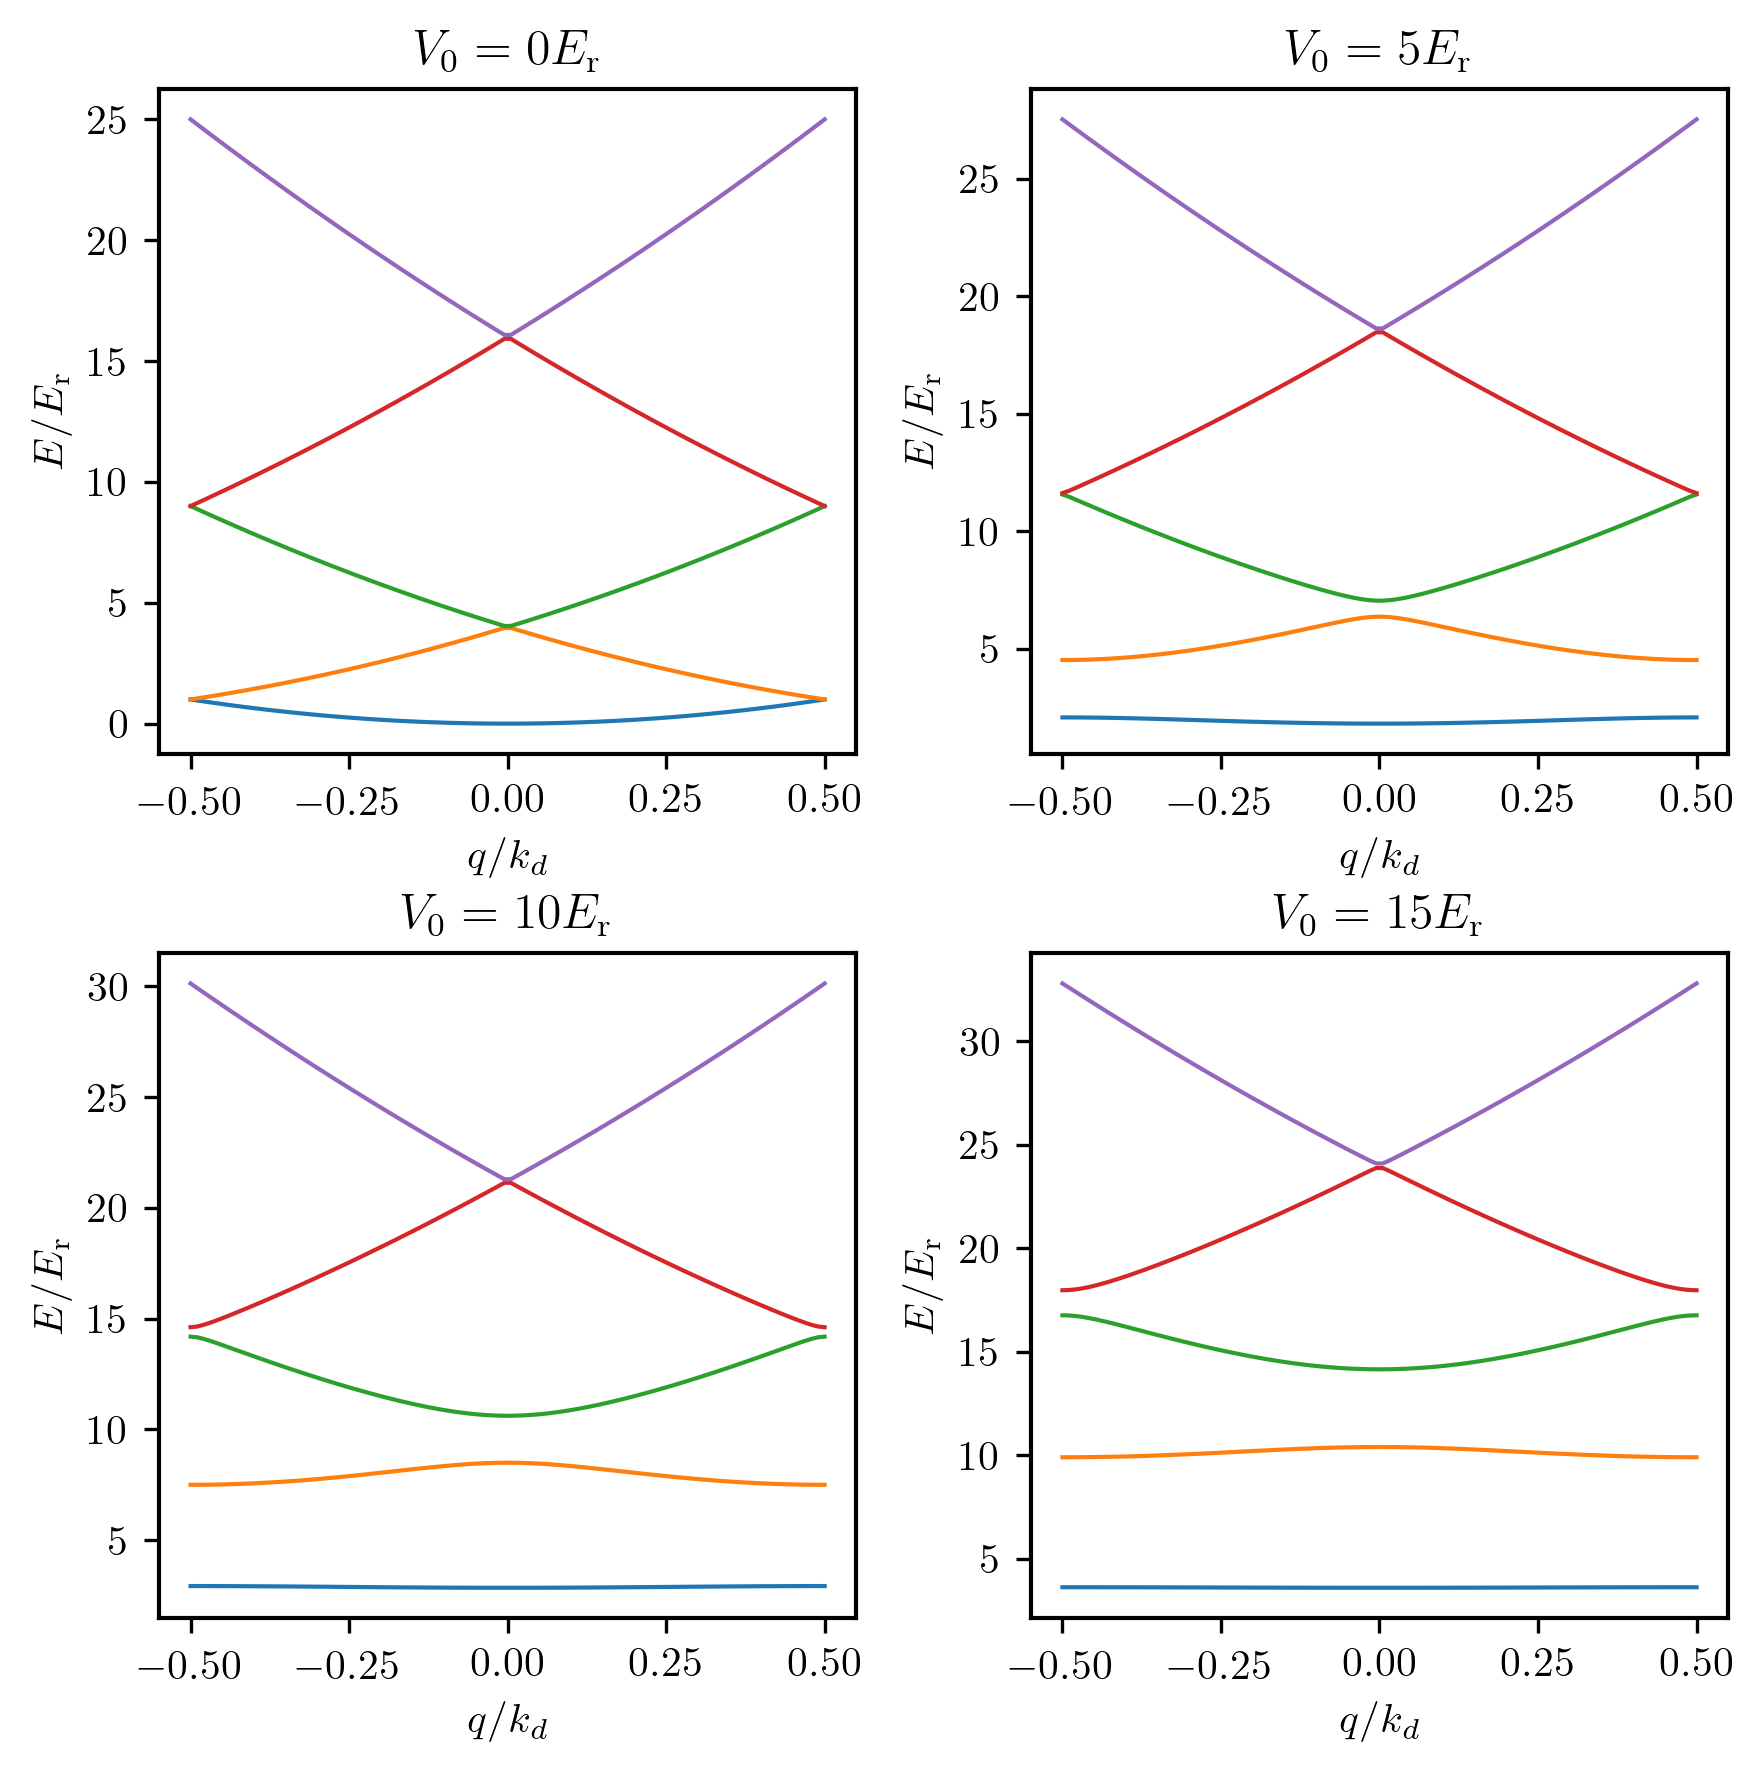
\includegraphics[width=\textwidth]{Fig/Chapter2/bloch_bands.png}
    \caption{First five Bloch energy bands for various lattice amplitudes $V_0$. The gap between the first bands increases as $V_0$ increases.}
    \label{fig:bloch_bands}
\end{figure}

In addition to the Bloch waves, it is possible to define a new kind of functions called the\textbf{ Wannier functions} \cite{wannier1937structure} that are localized near the lattice sites. They are defined from the Bloch waves by:

\begin{equation}
    w_{n, j}(x)=\sqrt{\frac{d}{2 \pi}} \int_{\mathrm{BZ}} \psi_{n, q}(x) e^{-i j q d} \mathrm{~d} q \quad, j \in \mathbb{Z}
    \label{eq:wannier_functions}
\end{equation}

\noindent with BZ denoting an integration over the first Brillouin zone and where $j$ can be interpreted as the index of a lattice site. Actually, we have from equation \ref{eq:wannier_functions} the simple relation:

\begin{equation}
    w_{n, 0}(x-j d)=w_{n, j}(x)
\end{equation}

The Bloch waves can then be re-written with the definition of the Wannier functions and write:

\begin{equation}
    \psi_{n, q}(x)=\left(\frac{d}{2 \pi}\right)^{1 / 2} \sum_{j} w_{n, j}(x) e^{-i j d q}
    \label{eq:bloch_as_wannier}
\end{equation}

The Bloch waves are then then sum of the localized Wannier function $w_{n, j}$ that can be interpreted as the wave-function of a particle located in lattice site $j$. The Hamiltonian of the system can also be re-written in terms of Wannier function. To do so, we start by writing it in the Bloch waves basis with the second quantification formalism, introducing the operator $\hat{b}_{n,q}$ that destroys a particle in the Bloch wave $\psi_{n,q}$.

\begin{equation}
    H_{1}=\sum_{n} \int_{\mathrm{BZ}} E_{n}(q) \hat{b}_{n, q}^{\dagger} \hat{b}_{n, q} \mathrm{~d} q
    \label{eq:H_bloch}
\end{equation}

To change into the Wannier function basis as defined in \ref{eq:bloch_as_wannier}, we introduce the operator $\hat{a}_{n,j}$ destroying a particle in the Wannier function $w_{n,j}$ and defined as:

\begin{equation}
    \hat{a}_{n}(q)=\sqrt{\frac{d}{2 \pi}} \sum_{j} \hat{b}_{n, j} e^{i j d q}
    \label{eq:a_wannier}
\end{equation}

\noindent Injecting equation \ref{eq:a_wannier} in equation \ref{eq:H_bloch}, we get:

\begin{equation}
    H_{1}=\sum_{n} \sum_{j, j^{\prime}} J_{n}\left(j-j^{\prime}\right) a_{n, j^{\prime}}^{\dagger} a_{n,j}
    \label{eq:H_Jn}
\end{equation}

\noindent This Hamiltonian has a nice physical meaning: it describes the tunneling process by which a particle in site $j$ can ``hop'' to another lattice site $j'$ with the tunneling amplitude $J_n (j-j')$ that writes:

\begin{equation}
    J_{n}\left(j-j^{\prime}\right)=\frac{d}{2 \pi} \int_{\rm{BZ}} e^{i\left(j-j^{\prime}\right) q d} E_{n}(q) \mathrm{d} q
\end{equation}

\noindent The probability for a particle to tunnel from lattice site $j$ to $j'$ is reduced as the distance between the two sites $j$ and $j'$ increases and as the potential barrier, \ie the lattice amplitude increases.

We will focus ourselves on the ground-state properties of the system and therefore assume that the lowest energy band is the only populated. This assumption is valid as long as $V_0 \geq 2.2 \ E_{\rm{E_r}}$ at which the gap is opening. In addition, for $V_0 \geq 3 \ E_{\rm{E_r}}$, we can use the tight-binding approximation for which only the tunneling events between adjacent sites are non-negligible. We simplify the Hamiltonian \ref{eq:H_Jn} by replacing  $J_{n}\left(j-j^{\prime}\right)$ by a constant $J$ denoting the probability to tunnel between adjacent lattice sites that we define as:

\begin{equation}
    J=-J_0(1)
\end{equation}

\noindent so that $J$ is positive. Finally, we obtain the first term of the Bose-Hubbard Hamiltonian:

\begin{equation}
    \hat{H}_1 = -J \sum_{\mean{i,j}} \hat{a}^{\dagger}_i \hat{a}_j
    \label{eq:H_band}
\end{equation}

\noindent where $\mean{i,j}$ denotes the ensemble of all adjacent lattice sites $i$ and $j$.

\subsubsection{Interaction term}
We now turn to studying the interaction term that we had left out in the full Hamiltonian of equation \ref{eq:H_lattice_full}. In the formalism of second quantification, the short-range, $s$-wave, 3D interaction Hamiltonian writes:

\begin{equation}
    \hat{H}_{\mathrm{int}}=\frac{1}{2} \int d x \int d x' U_{\mathrm{int}}\left(x, x'\right) \hat{\Psi}^{\dagger}(x) \hat{\Psi}^{\dagger}\left(x'\right) \hat{\Psi}\left(x^{\prime}\right) \hat{\Psi}(x)
\end{equation}

\noindent with $\hat{\Psi}(x)$ the operator destroying a particle at position $x$ that we write in terms of Wannier functions as:

\begin{equation}
    \hat{\Psi}(x)=\sum_{j} w_{j}(x) \hat{a}_{j}
\end{equation}

\noindent Note that we dropped the energy band number $n$ as we are studying the ground-state properties and thus only the lowest energy band. We approximate the interactions to be contact, repulsive interactions so that:

\begin{equation}
    U_{\rm{int}}= g \delta (x_1 - x_2)
\end{equation}

\noindent with $g$ the strength of the interactions. The interaction Hamiltonian can then be re-written:

\begin{equation}
    \hat{H}_{\mathrm{int}}=\frac{g}{2} \sum_{j_{1}} \sum_{j_{2}} \sum_{j_{3}} \sum_{j_{4}} a_{j_{4}}^{\dagger} a_{j_{3}}^{\dagger} a_{j_{2}} a_{j_{1}} \int w_{j_{4}}^{*}(x) w_{j_{3}}^{*}(x) w_{j_{2}}(x) w_{j_{1}}(x) \mathrm{~d} x
    \label{eq:h_int_intermediate}
\end{equation}

\noindent which is still a fairly complicated expression. We can however greatly simplify it by considering that the Wannier functions become narrower as the lattice depth increases. The overlap between the Wannier functions of the different lattice sites then becomes increasingly negligible. This means that the integral of equation \ref{eq:h_int_intermediate} is non zero only if $j_1=j_2=j_3=j_4$, \ie if we only consider on-site interactions. In the end, the interaction Hamiltonian writes:

\begin{equation}
    \hat{H}_{\rm{int}}=\frac{U}{2} \sum_j \hat{n}_j (\hat{n}_j -1)
\end{equation}

\noindent where we have introduced the on-site energy $U_{\mathrm{1D}}=g \int\left|w_{0,0}(x)\right|^{4} \mathrm{d}x$, easily generalized to the 3D case with $U=g \int(\left|w_{0,0}(x)\right|^{4} \mathrm{d}x)^3$. 

Combining this Hamiltonian to the non-interacting Hamiltonian of equation \ref{eq:H_band}, we reach the form of the famous \textbf{Bose-Hubbard Hamiltonian}:

\begin{equation}
    \hat{H}_{\mathrm{BH}}= -J \sum_{\mean{i,j}} \hat{a}^{\dagger}_i \hat{a}_j + \frac{U}{2} \sum_j \hat{n}_j (\hat{n}_j -1)
\end{equation}

\noindent Interestingly, the physics of the homogeneous ground-state depends on the two parameters $J$ and $U$ as we will see in the next paragraph. In particular, the ratio $U/J$ depends on the lattice depth $V_0$ that is easily controllable in an experiment, for instance by changing the power of the laser beams used to produce the lattice potential.


\section{The superfluid to Mott insulator transition}

We discuss in this section the properties of the Bose-Hubbard Hamiltonian ground-state for $N$ particles spread over $M$ sites, characterized by the ratio $U/J$ of the on-site interaction energy $U$ and the tunneling coefficient $J$. To begin, we will describe the extreme cases $U/J \to 0$ and $U/J \to \infty$, which are the only cases for which the Hamiltonian can be analytically solved. 

\subsection{Extreme cases}

\subsubsection{Perfect superfluid (SF) phase $\bm{U/J \to 0}$}

In this case, the particles are non-interacting. In these conditions, the ground-state $\ket{\Psi_0}$ of the N particles system is simply the product of the single particle ground state wave-function, \ie the Bloch wave-function for $q=0$:

\begin{equation}
    \ket{\Psi_0} = \frac{1}{\sqrt{N!}} (\hat{b}^{\dagger}(\bm{q}=0))^N \ket{0} = \frac{1}{\sqrt{N !}}\left(\frac{1}{\sqrt{M}} \sum_{j=1}^{M} \hat{a}_{j}^{\dagger}\right)^{N} \ket{0}
\end{equation}

\noindent In the thermodynamic limit with $N \to \infty$, $M \to \infty$, and the average filling defined as $\bar{n}=N/M$, it is possible to show at the price of a few lines of complex calculations \cite{gerbier_notes} that the probability to find $n_i$ atoms at a given site $i$ is:

\begin{equation}
    p\left(n_{i}\right) \approx e^{-\bar{n}} \frac{\bar{n}^{n_{i}}}{n_{i} !}
\end{equation}

\noindent We recognize the same Poissonian distribution that we would obtain for a bosonic coherent state as described in Chapter \ref{sec:chapter_1}. We can therefore write:

\begin{equation}
    \ket{\Psi_0} \approx |\Psi\rangle_{\mathrm{coh}}=\mathcal{N} e^{\sqrt{N} \hat{b}^{\dagger}(\bm{q}=0)} \ket{0} = \mathcal{N} \prod_{i} e^{\sqrt{\bar{n}} \hat{a}_{i}^{\dagger}} \ket{0} = \prod_{i} \mathcal{N}_{i} \sum_{n_{i}=0}^{\infty} \frac{\alpha_{i}^{n_{i}}}{\sqrt{n_{i} !}}\left|n_{i}\right\rangle_{i}
\end{equation}

\noindent with $\alpha_i=\sqrt{\bar{n}}$ and the normalization factor $\mathcal{N}_{i}=e^{-\left|\alpha_{i}\right|^{2} / 2}$. We thus find that the ground state can be described as a product of local coherent states associated to the lattice site $j$.

\section{Accessing the in-trap momentum distribution}

\subsection{The far-field regime}

\subsection{Mean-field interactions}

\subsection{Beyond mean-field interactions}

